\chapter[Development of methodologies to complement metagenomic sequencing for an integrative study of Ace Lake]{Development of methodologies to complement metagenomic sequencing for an integrative study of  Ace Lake}
\label{ch:ace}
\acresetall

%-----------------------------------------------------------------------------------------------
\section*{Co-authorship statement}
\addcontentsline{toc}{section}{Co-authorship statement}

Sections from this chapter have been published as:\\

Federico M. Lauro, Matthew Z. DeMaere, \textbf{Sheree Yau}, Mark V. Brown, Charmaine Ng,
David Wilkins, Mark J. Raftery, John A.E. Gibson, Cynthia Andrews-Pfannkoch, Matthew Lewis,
Jeffery M. Hoffman, Torsten Thomas, and Ricardo Cavicchioli. 
An integrative study of a meromictic lake ecosystem in Antarctica. \emph{\underline{The ISME Journal}} 
5:879--895, 2011.

I performed the metaproteomic mass spectral analysis, epifluorescence microscopy imaging,
microbial and viral counts and wrote the corresponding sections of the publication.

Contributions by others that support the work presented in this chapter are as follows.
Research was designed by Federico Lauro, Mark Brown, Torsten Thomas, John Gibson and Ricardo Cavicchioli.
Sample collection was performed by Federico Lauro, Mark Brown, Torsten Thomas, Jeffery Hoffman and Ricardo Cavicchioli.
\textsc{DNA} extraction and clone library preparation was performed by Cynthia Andrews-Pfannkoch and Jeffery Hoffman.
\textsc{DNA} sequencing quality control was performed by Matthew Lewis.
Metagenomic sequence filtering, mosaic assembly and annotation was performed by Matthew DeMaere.
Protein extraction, one-dimensional sodium dodecyl sulphate-polyacrylamide gel electrophoresis and liquid chromatography mass spectrometry and preliminary analysis performed by Charmaine Ng.
Assistance in mass spectrometry was provided by Mark Raftery.
\newpage

%----------------------------------------------------------------------------------------------
\section{Abstract}
Ace Lake is a saline meromictic lake and the most studied lake in the Vestfold Hills, Antarctica.
As a system of moderate biological complexity with extensive historic physical and chemical data, it was chosen as a site to implement an integrative study of the whole lake ecosystem.
Metagenomic analysis of Ace Lake revealed microbial taxa and metabolic genes were stratified according to the lake's water column structure and also was able to infer potential for nutrient cycling \cite{Lauro2011}.
%The aerobic mixolimnion resembles a marine surface water microbial community, the oxic--anoxic interface contains a near-clonal population of \ac{GSB} while the anoxic monimolimnion contains an extremely diverse assemblage that includes methanogenic \emph{Archaea} and \ac{SRB}.
%The viral signatures were detected at all depths of the lake, except for the \ac{GSB} layer \cite{Lauro2011}.

This study aimed to generate independent datasets complementary to metagenomic sequencing as part of the integrative analysis of the lake.
A method for visualising and enumerating cells and \acp{VLP} using epifluorescence microscopy was developed that does not require use of the relatively expensive Anodisc filters that were subject to an international drop in availability.
Microscopic examination confirmed the efficacy of the sequential filtration procedure used to size fractionate the lake microbiota.
Furthermore, it determined the densities of cells and \acp{VLP} and independently verified the absence of \acp{VLP} associated with the lake's \ac{GSB}.

Preliminary metaproteomic analysis of the Ace Lake depth profile using cross-species matching of mass spectra to the \ac{NR} yeilded few protein identifications \cite{Ng2010b}.
However, metaproteomic analysis of the \ac{GSB} layer using matching \ac{GSB} metagenomic sequences as the search database gave a 3-fold increase in protein identifications and allowed detailled description of the metabolism of the \ac{GSB} \cite{Ng2010a,Ng2010b}.
A metaproteomic analysis workflow was developed that similarly using metagenomes matched to the metaproteome samples as search databases and achieved substantial improvements in protein identification rates.
Application of the software package \textsc{Scaffold} 2.0 to protein mass spectral analysis was used to validate of protein identifications and allowed for protein abundance estimates using spectral counts.
Protein groups were identified that were overrepresented in each zone of the lake.
These data provided crucial to support a comprehensive description of the  entire Ace Lake ecosystem. 

%---------------------------------------------------------------------------------------------
\section{Introduction}
\acresetall
Ace Lake is a meromictic saline lake in the Vestfold Hills that separated from the sea $\sim$5,000 BP \cite{Bird1991}. 
Extensive physical, chemical and biological data has been collected from Ace Lake in the last decades \cite{Rankin1999}.
%This is summarised in the figure of the whole lake. %figure of lake.
The system is microbially-dominated and has reduced species diversity \cite{Bowman2000a} with the only metazoan life present being callanoid copepods. %Look up.
%What else? about the diversity from Bowman paper? Link to the intro.
Ace Lake is a highly stratified lake system that is 25 m at its deepest point \figref{fig:ace_diagram}.
\begin{figure}
\centering
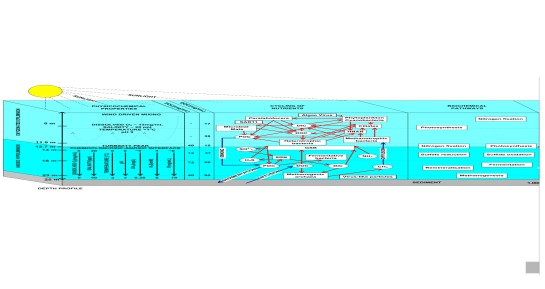
\includegraphics[width=\textwidth]{ace_figures/ace_diagram.pdf}
\caption[Physico-chemical and biological structure of Ace Lake]{Physico-chemical and biological structure of Ace Lake.
In the panel describing nutrient cycling biotic (red arrows) and abiotic (blue arrows) are shown.
The panel describing biochemical pathways shows the labels of the pathways at the depths where they are most significant.
The figure is adapted from \citet{Lauro2011}.
}
\label{fig:ace_diagram}

\end{figure}

It is ice-covered for $\sim$11 months of the year and generally thaws in January \cite{Rankin1999}.
Water is marine-derived and a largely neutral water balance has ensured salinity is close to that of seawater.
The lake is physically separated into an aerobic mixolimnion, a steep chemo/oxycline at 12.7 m and an anoxic monimolimnion.
The monimolimnion is sulfidic and methanogenic; both compounds have presumably accumulated through activity from \ac{SRB} and methanogenic archaea respectively \cite{Rankin1999, Lauro2011} \figref{fig:ace_diagram}.
As a physically and chemically well-characterised system of moderate diversity, Ace Lake was chosen as a model ecosystem to implement a whole systems level analysis to piece together ecosystem functioning.
Samples were obtained from the mixolimnion (5 and 11.5 m), the chemo/oxycline (12.7 m) and the monimolimnion (14, 18 and 23 m ).
Sampling was conducted according the design of the \ac{GOS} expedition \cite{Rusch2007} by using size fractionation of microbial biomass onto 3.0, 0.8 and 0.1 \textmu{}m membrane filters.
Both metagenomic and metaproteomic analysis was conducted on these samples to assess the taxonomic composition, the metabolic potential and identify the active members of the community.

From the metagenomic analysis significant differences were found in taxonomic composition between each size fraction and between the three zones of Ace Lake \cite{Lauro2011}.
The mixolimnion community is similar to a marine surface water assemblage consisting of a high abundance of the SAR11 clade of \emph{Alphaproteobacteria} related to ``\emph{Candidatus} Pelagibacter ubique'' and green algae of the order \emph{Mamiellales}.
However, diversity is reduced by one order of magnitude \cite{Lauro2011}.
Unlike Southern Ocean surface water, the mixolimnion is overrepresented in \emph{Cyanobacteria} related to \emph{Synechococcus} and \emph{Actinobacteria}, which may represent taxa that mark the transition from a marine to lake community.
A dense, near-clonal population of \acl{GSB} related to \emph{Chlorobium} termed \emph{C}-ace reside at the chemo/oxycline at 12.7 m \cite{Ng2010a, Lauro2011}.
Below, in the monimolimnion is a highly diverse community that includes \ac{SRB} and methanogenic \emph{Archaea}.
The viral community comprises \emph{Phycodnaviridae}, \emph{Myoviridae}, \emph{Siphoviridae}, \emph{Podoviridae} and unidentified viral families \cite{Lauro2011}. 
Bacteriophage sequences were abundant in the bottom waters, whereas the surface community, was dominated by phycodnaviruses \cite{Lauro2011}. 

Preliminary metaproteomic analysis along the vertical profile of Ace Lake has been performed using a cross species genomic database comprising the \ac{NCBI} \ac{NR} \cite{Ng2010b}.
A focused metaproteogeonomic analysis conducted on the dense \ac{GSB} layer using the matched \ac{GSB} metagenome as the database resulted in 3-fold increase in protein identifications compared to using the \ac{NR} database \cite{Ng2010b}.
%Put in a table of the rates of matches...
This indicates large gains in metaproteome coverage are possible using a matched metagenomic database \cite{Ng2010b}.
Significantly, \ac{GSB} appeared to be crucial in the lake ecosystem as they had the greatest genetic potential for nitrogen and carbon fixation as well as sulphur cycling \cite{Ng2010b, Lauro2011}.
Metaproteomic analysis was able to identify which proteins were actively expressed and thus the active pathways of the \ac{GSB} metabolism which are crucial to the function of the lake \cite{Ng2010a}.

This study aimed to develop and apply methodologies which provide independant data to complement an integrative metagenomic analysis of the whole Ace Lake ecosystem.
These included a modified epifluorescence microscopy procedure to determine cellular and viral densities and validate the efficacy of size-fractionation and a metaproteomic analysis workflow to identify proteins and estimate their abundance.

%---------------------------------------------------------------------------------------------

\section{Materials and methods}
\label{sec:ace_mm}
\subsection{Ace Lake samples}
Water samples were collected from Ace Lake (68$^{\circ}$28$'$23.2$''$S, 78$^{\circ}$11$'$20.8$''$E), Vestfold Hills, Antarctica on 21 and 22 December 2006. 
A hole positioned above the deepest point (25 m depth) of the lake was drilled through the 2 m ice cover of Ace Lake to reach the lake surface.
A volume of 1--10 L was collected by sequential size fractionation through a 20 \textmu{}m pre-filter directly onto 3.0, 0.8 and 0.1 \textmu{}m pore-size 293 mm polyethersulfone membrane filters \cite{Rusch2007}, along the depth profile.
Two independent sets of filters were obtained, one set for metagenomics and one for metaproteomics.
Filters were placed into sterile 50 ml tubes containing a solution of 2.5 mM EGTA, 2.5 mM EDTA, 0.1 mM Tris-EDTA (pH 8), 1mM PMSF (freshly prepared), 50 \textmu{}l protease inhibitor cocktail VI (Calbiochem, San Diego, \textsc{CA}, \textsc{USA}) and the tubes placed in liquid nitrogen before storage at $-$80$^{\circ}$C.
The protease inhibitor cocktail has a broad specificity for inhibition of serine, cysteine, aspartic and metalloproteases within protein extracts.
Samples were taken in the order, 23, 18, 14, 12.7, 5 and finally, 11.5 m.

After samples from each depth were collected, the sample racks were sequentially washed with 2 $\times$ 25 L 0.1 N NaOH, 2 $\times$ 25 L 0.053\% NaOCl, and 2 $\times$ 25 L fresh water. 
The sample hose was flushed with water from each depth before being applied to the filters. 
A \emph{Chlorobium} signature was identified at 5 m, but not immediately above the \ac{GSB} layer at 11.5 m. 
As the next sample taken after sampling at 12.7 m was at 5 m, and then 11.5 m, despite all equipment being thoroughly washed with bleach, NaOH and water, 
the simplest explanation for the \ac{GSB} signature at 5 m is carry-over from sampling of the dense biomass at 12.7 m. 

A sonde probe (\textsc{YSI} model 6600, \textsc{YSI} Inc., Yellow Springs, \textsc{OH}, \textsc{USA}) was used to record depth, dissolved oxygen content, pH, salinity, temperature and turbidity throughout the water column of the lake. 
Total organic carbon was determined using a total organic carbon analyzer, TOC-5000A (Shimadzu, Kyoto, Japan) equipped with a \textsc{ASI}-5000A auto sampler (Shimadzu), and particulate organic carbon by standard protocols 
\url{(http://www.epa.gov/glnpo/lmmb/methods/about.html)} 
at the Centre for Water and Waste Technology, \textsc{UNSW}.

\subsection{\textsc{DNA} extraction, sequencing and data cleanup}
\textsc{DNA} extraction and Sanger sequencing was performed on 3730xl capillary sequencers (Applied Biosystems, Carlsbad, \textsc{CA}, \textsc{USA}) and pyrosequencing on \textsc{GS20 FLX} Titanium (Roche, Branford, \textsc{CT}, \textsc{USA}) at the \acl{JCVI} in Rockville, \textsc{MD}, \textsc{USA} \cite{Rusch2007}. 
The scaffolds and annotations will be available via \ac{CAMERA} and public sequence repositories such as the \ac{NCBI} and the reads will be available via the \ac{NCBI} Trace Archive. 

Sanger reads were trimmed according to quality clear ranges.
The quality of pyrosequencing reads was assessed as follows: 
a \ac{BLAST} nucleotide database was created from the Sanger reads of the 0.1 \textmu{}m fraction of samples GS230, GS231 and GS232 (see \tabreft{tab:ace_metag} for summary of the metagenomic data and sample IDs).
\input{ace_figures/ace_metag.tex}
After performing a \ac{BLAST} comparison of the corresponding pyrosequencing reads against each Sanger sequence database with a minimum bitscore of 80 and maximum e-value of 0.1, reads were binned according to length.
The percentage of reads for each bin lacking a match to the Sanger read database was recorded. 
The percentage reads at least 25\% repetitive after \textsc{MDUST} \cite{Morgulis2006} analysis at default settings, and the percentage of reads containing N's, were assessed. 
In contrast to earlier pyrosequencers \cite{Huse2007}, no length-dependent bias in reads containing N's was observed. 
However, short reads had a disproportionately high number of repeats. 
Moreover, based on the proportion of reads with no match to the Sanger data set, both very short and very long reads had a disproportionately high number of errors; an observation that was previously reported \cite{Huse2007}.

On the basis of this analysis, a three step filtering process was applied to each sample. 
Reads were initially run through the Celera \textsc{sffToCA} \cite{Miller2008} pre-processor followed by \textsc{Lucy} \cite{Chou2001} and finally, excluding the bottom 8\% and top 3\% of reads determined from the read length distribution. 
As the \textsc{sffToCA} (v5.3) pre-processor removes all reads with a perfect prefix of any other read it overcomes the `perfect duplicates' problem \cite{Gomez-Alvarez2009}.
 
After this process, $<$5\% of the reads belonged to clusters of duplicates with three or more reads, and \ac{COG} of proteins classification of these reads showed an over-representation of category L (replication, recombination and repair) that includes mobile genetic elements, which are often duplicated, suggesting a potential biological significance for the duplicated reads. 
It is possible these residual duplications are a result of high gene copy number or localized fragility of DNA sequences that might be biasing the shear points.

\subsection{Metagenomic DNA assembly and annotation}
Mosaic assemblies were generated for each sample fraction using Celera \ac{WGS} Assembler v5.3 \cite{Myers2000}. 
For each assembly, the runtime parameters used were as outlined for 454 sequencing data in the published standard operating procedure\\ 
\url{(http://sourceforge.net/apps/mediawiki/wgs-assembler/index.php?title 1⁄4SFF\_SOP)}. 
As none of the samples can be considered clonal, these are regarded as stringent assemblies \cite{Rusch2007}. 
Each 0.1 \textmu{}m fraction assembly was a hybrid of Sanger and 454 read data, wherein the estimated genome size was manually set to minimize the number of unitigs from abundant organisms being falsely classified as degenerate \cite{Rusch2007}. 
Annotation of each sample fraction assembly was carried out using an in-house pipeline, wherein the pipeline stages consisted of genomic feature detection and subsequent annotation \cite{DeMaere2011}. 
Detected features consisted of \acp{ORF}, transfer \textsc{RNA} and \ac{rRNA}. 
Each detected \ac{ORF} was further annotated by \ac{BLAST} comparison against \ac{NR}, Swissprot and \ac{KEGG}-peptide sequence databases and by \ac{HMMER} comparison against \ac{TIGRFAM} \cite{Haft2001}, \ac{COG} \cite{Tatusov1997, Tatusov2003} and known marker genes \cite{vonMering2007}.
In all cases the cut-off e-value was a maximum of 1e$-$5. 


\subsection{Epifluorescence microscopy}
Samples of unfiltered lake water and the flow-through from 3.0 and 0.8 \textmu{}m filters from all depths were collected on November 2008 and fixed on site in formalin 1\% (v/v). 
The samples were stored at $-$80$^{\circ}$C for subsequent direct counts of cells and \acp{VLP}. 
Enumeration was performed according to the method of \citet{Patel2007} with modifications. 
Lake water samples were filtered onto 0.01 \textmu{}m pore-size polycarbonate filters (25 mm Poretics, \textsc{GE} Osmonics, Minnetonka, \textsc{MN}, \textsc{USA}). 
Filters were air dried, then placed with the back of the filter on top of a 30 ml aliquot of 0.1\% (w/v) molten low-gelling-point agarose and allowed to dry at 30$^{\circ}$C. 
Samples were stained by the addition of 2 \textmu{}l working solution (1 in 400 dilution in 0.02 \textmu{}m filtered sterile Milli-Q) of \textsc{SYBR} Gold (Molecular Probes, Eugene, \textsc{OR}, \textsc{USA}) to 20 \textmu{}l of mounting medium (\textsc{VECTASHIELD} HardSet, Vector Laboratories, Burlingame, \textsc{CA}, \textsc{USA}). 
Stained samples were counted immediately.
Samples were visualised under wide-blue filter set (excitation 460--495 nm, emission 510--550 nm) with an epifluorescence microscope (Olympus BX61, Hamburg, Germany).


\subsection{Protein extraction}
Proteins were extracted from membrane filters from all 0.1 \textmu{}m fractions from the six depths (5, 11.5, 12.7, 14, 18 and 23 m) according to the protocol developed by \citet{Ng2010a}, which is as follows.
The 0.1 \textmu{}m filters were allowed to thaw at room temperature and cut into quarters asceptically.
Separate extractions were performed on each filter quarter which served as technical replicates.
Each quarter filter was suspended in a lysis buffer containing 10mM Tris-EDTA (pH 8), 20 \textmu{}l of protease inhibitor cocktail VI (Calbiochem), 0.1\% sodium dodecyl sulphate, and 1 mM dithiothreitol.
Three freeze-thaw cycles were performed using liquid nitrogen.
The membrane was then removed, and the buffer was subject to five cycles of sonication of 40 s on a 30 \% duty cycle at power setting of 3, which serves to lyse any remaining cells and shear nucleic acids.
The mixture was centrifuged at 5000 \emph{g} for 25 min at 4$^{\circ}$C to remove insoluble material.
Smaller insoluble particles were removed by filtration through a 0.22 \textmu{}m syringe filter (Millipore, Sydney, NSW, Australia).
Buffer exchange with 30 ml of 10 mM Tris-EDTA (pH 8) and concentration of soluble extracted proteins was performed in a 5 kDa cut-off Amicon Ultra-15 filter unit (Millipore).
Protein concentration was determined using a bicinchoninic acid protein assay kit (Sigma-Aldrich, Sydney, NSW, Australia).

\subsection{Metaproteomic \acs{1D-SDS PAGE} and \acs{LC}-\acs{MS-MS}}
Extracted proteins were separated by \ac{1D-SDS PAGE} containing 12 \% SDS using a Mini-PROTEAN system (Bio-Rad, Sydney, NSW, Australia) as described previously \cite{Saunders2006}.
Trypsin digestion, \ac{LC} and mass spectrometry was conducted according to \citet{Ng2010a} as follows.
The gels were silver stained and the images acquired with a UMAX PowerLook 1000 flat-bed scanner (Fujifilm, Berthold, Vic, Australia).
Each lane containing the size separated proteins were excised and sliced according to size with a sterile scalpel.
Gel slices were washed in sterile Milli-Q water followed by acetonitrile, then subject to a series of reductioin, alkylation and dehydration reactions.
Digestion of proteins with trypsin was conducted by rehydrating gel pieces in a buffer of 200 ng trypsin (Promega, Sydney, NSW, Australia) and 10 mM NH$_4$HCO$_3$ at 37$^{\circ}$C overnight. 
Gel slices were dehydrated in acetonitrile in a centrifugal evaporator (SpeedVac).

Peptides were rehydrated in 1\% formic acid and 0.05\% heptafluorobutyric acid and separated by nano \ac{LC} using an Ultimate 3000 \acs{HPLC} and autosampler system (Dionex, Amsterdam, the Netherlands).
Samples of 2.5 \textmu{}l were concentrated and desalted onto a micro C18 precolumn (500 \textmu{}m $\times$ 2 mm; Michrom Bioresources, Auburn, \textsc{CA}, \textsc{USA}) with H$_2$O:CH$_3$CN (98:2, water to 0.05\% heptafluorobutyric acid) at 20 \textmu{}l min$^{-1}$.
After a 4 min wash, the precolumn was switched into line (Valco 10 port valve; Dionex) with a fritless nano column (75 \textmu{}m $\times$ 10 cm) containing C18 medium (5 \textmu{}, 200 \AA\ Magic, Michrom).
Peptides were eluted using a linear gradient of H$_2$O:CH$_3$CN (98:2, 0.1\% formic acid) to H$_2$O:CH$_3$CN (63:36, 0.1\% formic acid) at 350 nl min$^{-1}$ over 30 min.

1800 V was applied to the low volume tee (Upchurch Scientific, Oak Harbor, \textsc{WA}, \textsc{USA}) and the column tip was positioned $\sim$0.5 cm from the heated capillary (250$^{\circ}$C of an LTQ-FT Ultra mass spectrometer (Thermo Electron, Bremen, Germany).
Positive ions were generated by electrospray and the LTQ-FT Ultra was operated in data-dependent acquisition mode.
A survey scan \emph{m/z} 350--1,750 was acquired in the FT ICR cell (resolution $=$ 1,000,000 ions in the linear ion trap).
Up to the six most abundant ions ($>$3,000 counts) with charge states of $+$2, $+$3 or $+$4 were sequentially isolated and fragmented within the linear ion trap using collision-induced dissociation with an activation $q$ $=$ 0.25 and activation time of 30 ms at a target mass value of 30,000 ions.
\emph{m/z} ratios selected for \ac{MS-MS} were dynamically excluded for 30 s.
Peak lists were generated using \textsc{extract\_msm} from \textsc{Mascot Daemon} (Matrix Science, Thermo, London, \textsc{UK}) using the default parameters.

\subsection{Mass spectra analysis and validation of metaproteomic identifications}
The specta generated from \ac{MS} were searched against the protein sequence database corresponding to that depth constructed from the 0.1 \textmu{}m mosaic assemblies using \textsc{Mascot} version 2.1 (Matrix Science).
\textsc{Mascot Distiller} (Applied Biosystems) was used as the data import filter with the following criteria applied to the \ac{MS-MS} ion search: a maximum of one missed cleavage for trypsin, peptide mass tolerance of $\pm$ 4 ppm, a fragment mass tolerance of $\pm$0.6 Da and variable modifications of acrylamide, carbamidomethyl and oxidation.
The number of protein sequences in each database were as follows: 5 m, 138,208; 11.5 m, 133,948; 12.7 m, 27,142; 14 m, 62,436; 18 m, 71,512; and 23 m, 128,878. 
\textsc{Scaffold} 2.0 (version Scaffold\_2\_05\_01, Proteome Software Inc., Portland, \textsc{OR}, \textsc{USA}) was used to validate \ac{MS-MS}-based peptide and protein identifications. 
Peptide and protein identifications were accepted if they could be established at $>$95\% and 99\% probability, respectively, as specified by the \textsc{Peptide Prophet} algorithm \cite{Keller2002}. 
Protein identifications required the identification of at least two peptides.
 
Proteins that contained similar peptides and could not be differentiated based on \ac{MS-MS} analysis alone were grouped to satisfy the principles of parsimony and are referred to as a protein group. 
Spectral counting was used to semi-quantitively estimate protein abundance. 
The total assigned spectra that matched to each identified protein were exported from \textsc{Scaffold} 2.0. 
For similar proteins that have shared peptides (a protein ambiguity group), spectra were assigned to the protein with the most unique spectra. 
To normalise for variation in total spectra acquired between sample replicates, the number of spectra of each protein was multiplied by the average total spectra divided by the total spectra of the individual replicate. 
The spectral count of each protein was averaged across the replicates. 
As longer proteins are more likely to be detected, the average spectral counts were divided by the length of the protein. 
This value is equivalent to the normalised spectral abundance factor \cite{Florens2006, Zybailov2006}. 
In order to compare the relative abundance of proteins between depths, the normalised spectral abundance factor was divided by the average read depth of the contig (scaffold or degenerate) to which the protein mapped. 

If $>$90\% of a scaffold’s length consisted of surrogate (highly degenerate unitig) sequence, the average read depth of the surrogate was used. 
For identified proteins that were part of a protein group the longest protein length and largest read depth value in the group was used. 
Pairwise comparisons of each zone were conducted on \ac{COG} assigned proteins. 
The normalised spectral counts from each protein was aggregated based on their \ac{COG} annotation. 
All proteins that were part of an ambiguity group were confirmed to share the same \ac{COG} annotation to ensure counts were not biased because of the common spectra.

The summed spectral counts from 5 and 11.5 m (mixolimnion), and 14, 18 and 23 m (monimolimnion) were pooled. 
Statistical significance of differences between each zone was assessed using Fisher's exact test, with confidence intervals at 99\% significance calculated by the Newcombe–Wilson method and Holm-Bonferroni correction (p-value cutoff of 1e$-$5) in \ac{STAMP} \cite{Parks2010}. 
All proteins identified, including their gene identifier, normalised spectral abundance, \ac{COG} and \ac{KEGG} Orthology identifiers, \ac{KEGG} locus tag and matching \ac{COG} or \ac{KEGG} description are provided in the Appendix \tabreft{tab:ace_protids_5m}--\tabreft{tab:ace_protids_23m}.



%---------------------------------------------------------------------------------------------

\section{Results and discussion}

\subsection[Development of an epifluorescence microscopy methodology]{Development of an epifluorescence microscopy methodology}
An epifluorescence microscopy methodology was developed to allow examination of cellular morphology and enumeration of cells and \acp{VLP} in Ace Lake.
Development of a revised method was necessary due to inability to source 25 mm diameter 0.02 \textmu{}m pore-size Anodisc filters (Whatman) that have been long used with fluorescent nucleic acid dyes for this purpose \cite{Hennes1995, Noble1998, Patel2007}. 
They were marked for discontinuation in December 2008 after the take-over of Whatman by \textsc{GE} Healthcare and was the cause of a global shortage that was strongly opposed by the viral ecology community \cite{Torrice2009}.
Since conducting this research, supply of 25 mm Anodisc filters has resumed, albeit at much greater cost per filter. 
The need to develop alternative methodolodies has been great enough that protocols were developed independently by other research groups \cite{Budinoff2011, Diemer2012} stressing the utility of alternatives.

Clear \ac{PCTE} membrane filters were selected for use as a viable alternative product as they have a defined pore-size of sufficiently small diameter (0.01 \textmu{}m) to capture \acp{VLP}. 
Furthermore, they have been used in early studies for \acp{VLP} enumeration \cite{Hara1991, Proctor1992}, have a long history of use with the enumeration of cells \cite{Hobbie1977} and therefore require no new materials to be easily adopted for use.
Finally, use of \ac{PCTE} membranes is approximately 10 times cheaper than the use of Anodiscs and are not subject to drops in availability.
However, \ac{PCTE} membranes have several reported shortcoming that have precluded their standard use for viral enumeration.
The 0.01 \textmu{}m 25 mm \ac{PCTE} filters are difficult to handle compared to 25 mm Anodisc filters that have a plastic support ring around the edge.
Also, \ac{PCTE} filters appear to have higher background fluorescence, have a slow flow-rate taking $\sim$1--1.5 hours to filter 2 ml \cite{Hara1991} and have been reported to give \ac{VLP} counts an order of magnitude lower than that of Anodiscs \cite{Budinoff2011}.%more ref?

The protocol used is detailled in section \ref{sec:ace_mm} \emph{Materials and methods} where the main challenges of using \ac{PCTE} were overcome for the purposes required for this study.
0.01 \textmu{}m pore-size \ac{PCTE} filters can form creases or wrinkles when mounted in the glass vacuum filter.
Good placement of the \ac{PCTE} filter was achieved by touching the edge of the \ac{PCTE} filter against the damp backing filter, making sure it was aligned and then gently and evenly releasing it in a single direction. 
0.01 \textmu{}m pore-size \ac{PCTE} filters also easily become statically charged and will become attracted to surfaces so careful handling is required during manipulation. 
The greatest drawback in the use of \ac{PCTE} filters of such small pore-size is they similarly have a tendency to crinkle when mounted on the glass slide that can make visualisation of cells and \acp{VLP} on a single focal plane difficult.
Agarose was used to embed the filters to help flatten the membrane and aid in mounting.
However, this was not strictly necessary if filters are dried well and pressed flat against the glass slide with a minimal volume of mountant.
Even though careful handling is possible, this method likely requires more technical replicates than Anodisc filters because any \acp{VLP} outside the focal plane will not be counted.
Furthermore, as similarly reported by \citet{Diemer2012} for 0.03 \textmu{}m \ac{PCTE} membranes, distribution of \acp{VLP} on the membrane appears more variable than for Anodiscs with local regions devoid of \acp{VLP} and others with pooling of \acp{VLP}.
The patchier \acp{VLP} distribution was attributed to greater irregularity in pore distribution compared to that of Anodisc filters and was considered to be the main contributing factor to variability in \ac{VLP} counts \cite{Diemer2012}

Back ground fluorescence was at an acceptable level when the SYBR Gold stain is only incorporated into the mountant after filtration rather than staining in the column.
This is one key difference between this protocol and others that use \ac{PCTE} membranes \cite{Hara1991, Proctor1992, Diemer2012}.
Other protocols have used 0.08 \textmu{}m membranes pre-stained with Irgalan Black \cite{Proctor1992} or 0.03 \textmu{}m pre-stained with Sudan black B \cite{Diemer2012} to minimise background fluorescence.
Pre-staining of 0.01 \textmu{}m membranes would be an option for future optimisation of this protocol.

Only one prior report of filtration of natural water onto the \ac{PCTE} membranes with 0.01 \textmu{}m pore-size was found \cite{Hara1991}.
Such a small pore-size necessitates a very strong seal of the filter column against the glass base with no air leaks.
Leakage can be eliminated by sealing the fritted base to the column with laboratory film. 
However, the slow flow-rate was not a property of these \ac{PCTE} filters that could be overcome.
As the filtration and visualisation was performed on fixed samples in the laboratory rather than in the field, the time taken for filtration of 2--3 hours for each sample was not deemed problematic for the purposes of this study.
Counts of \acp{VLP} have been shown to decrease dramatically with time even when preserved with aldehyde-based fixatives \cite{Wen2004}.
Collecting larger sample volumes and flash freezing in liquid nitrogen and storing at $-$80$^{\circ}$C helps to slow this effect \cite{Patel2007}.
Due to logistic contraints of working in the Antarctic, counts in the field were not possible so \ac{VLP} counts are expected to be underestimated.
However, all samples were processed within a similar time frame so the relative \ac{VLP} abundances down the depth profile and between size fractions are expected to be accurate as all samples would have undergone comparable amounts of \ac{VLP} loss. 

Overall, a viable alternative methodology was successfully developed for visualisation and enumeration of cells and \acp{VLP} using \ac{PCTE} membrane filters for use in this study \figref{fig:ace_microscopy}.
\begin{figure}
\includegraphics[width=\textwidth]{ace_figures/ace_microscopy.jpg}
\caption[Epifluorescence microscopy of Ace Lake microbiota]{Epifluorescence microscopy images of Ace Lake microbiota. Scale bar $=$ 20 \textmu{} m. ND, not determined.
}
\label{fig:ace_microscopy}

\end{figure}

To be a competitive alternative to Anodisc filters in terms of enumeration accuracy, further work is required that compares counts using this methodolody and the current standard Anodisc-based protocol \cite{Patel2007} with viral samples of known densities.

%------------------------------------------------------------------------------------------------------------------------

\subsection[Community stratification supported by cell and \acs{VLP} densities]{Size and depth stratification of the community supported by cell and \acs{VLP} densities}

Epifluorescence microscopy images of Ace Lake microbiota showed a clear decrease in larger and particularly filamentous cells between filter size fractions \figref{fig:ace_microscopy}.
The sequential filtration of suspended microbial biomass from aquatic environments has been utilised as part of the landmark Sargasso Sea metagenomic study \cite{Venter2004} and \ac{GOS} expedition \cite{Rusch2007}.
The Ace Lake samples were collected using the same sampling strategy as the \ac{GOS} dataset but has sequence information from all three filter sizes and was able determine if size fractionation is effective at separating the microbial community and if functional differences are associated with size.
Both taxonomic and functional gene composition were shown in the metagenomic analysis to differ significantly with size fraction, particularly between the 0.1 \textmu{}m and the larger size fractions, indicating resource partitioning in the community \cite{Lauro2011}.
The clear difference between the size fractions indicated the sequential filtration process is an effective means to separate the community and that different sized populations in the community have different ecological roles (\emph{e.g.} particle attached copiotrophs or planktonic oligotrophs).
For example, \emph{Flavobacteria} were only detected in the 3.0 \textmu{}m size fraction mixolimnion metagenomes and were inferred to be involved in mineralisation of particulate matter \cite{Lauro2011}.
This correlates with the absence of larger, particularly long rod shaped cells, in the $>$0.8 \textmu{}m microscopic image \figref{fig:ace_microscopy} indicating these larger cells are likely to be copiotrophic \emph{Flavobacteria} involved in degradative processes.
Depth was another variable which strongly drove differences in the Ace Lake community \cite{Lauro2011}.
This was again evident in the microscopy images that show the appearance of long filamentous cells only in the monimolimnion samples \figref{fig:ace_microscopy}.

Cell and \ac{VLP} densities are not obtainable from metagenomic sequence data and necessitates an independent method of determination.
The first studies to determine viral densities in natural systems found that viruses are the most numerous biological entities on the planet and likely play a large role in plankton mortality in the ocean \cite{Bergh1989,Proctor1990}. 
\ac{VLP} counts from marine environments vary with depth and trophic status ranging from 10$^6$ to 10$^8$ \acs{VLP} ml$^{-1}$ \cite{Suttle2005}.
%\ac{VLP} counts from lakes in the Vestfold Hills appear to increase with salinity \cite{Laybourn-Parry2001}.
Both cellular and \ac{VLP} counts are linked with environmental factors such as trophic status \cite{Lauro2009}. 
Enumeration of cells and \acp{VLP} in Ace Lake showed cell densities were lowest in the relatively oligotrophic mixolimnion (0.8--1.3 $\times$ 10$^6$ cell ml$^{-1}$) and were by an order of magnitude higher in the copiotrophic monimolimnion (1.6 $\times$ 10$^7$ cell ml$^{-1}$ in the 23 m sample) \figref{fig:ace_counts}.
\begin{figure}
\centering
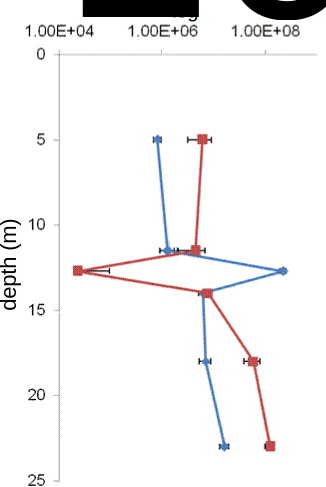
\includegraphics[width=50mm]{ace_figures/ace_counts.pdf}
\caption[Counts of microbial cells and \acs{VLP}s in Ace Lake]{Counts of microbial cells (blue) and \acs{VLP}s (red) by epifluorescence microscopy along a depth profile of Ace Lake.
Error bars represent one standard deviation.
No \acp{VLP} were detected at 12.7 m depth and the value reported represent the detection limit of the counting procedure (\emph{i.e.} one \acs{VLP} detected in one field of view).
}
\label{fig:ace_counts}

\end{figure}

Cell densities were highest at 12.7 m (2.2 $\times$ 10$^8$ cells ml$^{-1}$) corresponding to the \ac{GSB} layer.


\ac{VLP} abundance was consistently higher than the cellular counts but the ratio of \ac{VLP} to cells ranged throughout the water column from $\sim$1--8.5.
The exception to this was the 12.7 m where there was an unusual lack of \acp{VLP} \figref{fig:ace_counts}.
These data corresponded with the metagenomic data from 12.7 m that found no viral signatures associated with the \ac{GSB} at the chemo/oxycline \cite{Lauro2011}.
From metagenomic data alone the absence of viral signatures in the metagenome does not preclude the presence of viruses with ss\textsc{DNA} or \textsc{RNA} genomes that would not be detected by \textsc{DNA} sequencing method used.
Epifluoresence microscopy using SYBR Gold nucleic acid stain would in principle detect \acp{VLP} containing non-dsDNA genomes \cite{Patel2007} that would otherwise be missed in the metagenome.
\figreft{fig:virus_compare} contrasts the epifluorescence images of water from 5 m sample with the 12.7 m sample confirming the lack of visible \acp{VLP} in the latter.
\begin{figure}
\includegraphics[width=\textwidth]{ace_figures/virus_compare.pdf}
\caption[Lack of \acs{VLP} in 5 m and 12.7 m Ace Lake samples]{Epifluorescence microscopy images contrasting Ace Lake water samples from (\textbf{A}) 5 m and (\textbf{B}) 12.7 m. 
Numerous \acp{VLP} are evident in the 5 m sample, but not in the 12.7 m sample. Scale bar $=$ 20 \textmu{}m.
}
\label{fig:virus_compare}

\end{figure}

This provided independent support that the \ac{GSB} population in Ace Lake represents an exception to viral--bacterial population dynamics that describes high rates of genotype cycling in aquatic systems \cite{Rodriguez-Brito2010}.


%---------------------------------------------------------------------------------------------

\subsection[Development of a metaproteomic mass spectra analysis workflow ]{Development of a metaproteomic mass spectra analysis workflow }

Identification of proteins from a microbial community (metaproteomics) indicates which populations or processes are active in the environment and is thus a powerful tool for understanding ecosystems.
However, protein identification by the `shotgun' proteomics approach favoured in metaproteomics \cite{Ram2005} is computationally challenging.
The general shotgun proteomics workflow in \figreft{fig:workflow} shows that apart from successful sample preparation to simplify the complex protein mixture, protein identification depends greatly upon the post-\ac{MS} bioinformatic analysis.
\input{ace_figures/workflow.tex}
This is due to how the \ac{MS-MS} data are used to identify proteins (see \citet{Marcotte2007} for a primer on shotgun proteomic identification).

Briefly, the peptides from digested proteins are separated by \ac{LC} and subject to a round of mass spectra acquisition where the mass of the peptides (precursor ions) are detected.
Selected peptides undergo collision-induced dissociation where they fragment preferentially at the peptide bond.
A second round of mass spectra is acquired of the peptide fragments (fragment ion spectra) that represents the amino acid sequence of the peptide.
An \emph{in silico} enzymatic digestion is performed on a genomic database to predict the precursor ion masses and their corresponding fragment ion spectra.
The fragment ion spectrum and precursor ion mass is used to determine the most likely amino acid sequence of the peptide by comparison to the genomic database and thereby identify the protein(s) of origin.
Since spectral matching depends on extremely high mass sensitivity, the ideal genomic database contains complete coverage of sequences from the organism(s) from which the proteins originated. 
A single amino acid change is sufficient for a peptide match to fail although matching is tolerant to synonymous changes.

Preliminary metaproteomic analysis was conducted on the 0.1 \textmu{}m fraction samples along the depth profile of Ace Lake using sequences from \ac{NR} as the search database \cite{Ng2010b} as metagenomic data were not yet available.
The use of a cross-species database requires the genomes to be sufficiently related to identify proteins and application of stringent statistial cut-off to avoid false-positive matches.
Across all six samples, a total of 10,443 peptides were identified corresponding to 308 proteins from $\sim$400,000 \ac{MS-MS} spectra \cite{Ng2010b}.
Rates of protein identification were low compared to a similar metaproteomic analysis of the Sargasso Sea, which achieved  a total of 5,501 peptide identifications corresponding to 1,042 proteins from $\sim$30,000 \ac{MS-MS} spectra \cite{Sowell2009}. 
This indicated that the Ace Lake community was sufficiently different from relatives in the \ac{NR} database to achieve high rates of protein identification.
A key difference in the Sargasso Sea study was the inclusion of metagenomic sequence in the search database from their target populations of SAR11, \emph{Synechoccocus}, and \emph{Prochlorococcus} \cite{Sowell2009}.
The low identification rate was to be expected as it has been shown that only half the number of proteins are identifiable when using a genomic database that shares 90\% amino acid identity with the matching genome \cite{Denef2007}.

Once the metagenomic sequence for the \ac{GSB} layer became available, re-analysis of the mass spectra to the matched \ac{GSB} metagenome was performed as this sample had the lowest genomic complexity and was expected to obtain high identification rates \cite{Ng2010a, Ng2010b}.
In the re-analysis, 3,970 peptides were identified, mapping to 504 proteins from $\sim$100,000 spectra, which was a near 3-fold increase in the number of protein identifications \cite{Ng2010a, Ng2010b}.
This indicated a similar increase in protein identifications could be achieved with the other Ace Lake samples.
However, metagenomic sequence from more diverse communities adds additional bioinformatic considerations for protein matching due to their inherently greater heterogeneity.
For a protein to be identified according to standard stringency cut-offs it requires at least two peptides to be mapped to it with at least one of those being unique. 
The converse of this is that it allows for the fact there are potentially non-unique peptides shared by other proteins.
Although shared peptides occur between proteins in single genomes, a typical metagenome will contain related species or strains and therefore many more copies of closely related proteins.
%This greatly decreases the probability of finding a unique peptide and thus can exclude proteins from identification.
Protein identification scores in the focussed \ac{GSB} study was also set to only accept identifications above a determined \ac{FDR}.
This is the score given by a peptide match to a randomised version of the genomic database \cite{Ng2010a, Ng2010b}.

To address the additional challenges posed by higher diversity metagenomic data, the program \textsc{Scaffold} 2.0 was adopted for the filtering and validation of peptide and protein matches \figref{fig:workflow}. 
Instead of determining a \ac{FDR}, \textsc{Scaffold} 2.0 employs the \textsc{Peptide Prophet} algorithm \cite{Keller2002} for protein validation.
This algorithm fits a distribution of scores from correct and in-correct peptide matches and from this calculates the probability that each result is a genuine match \cite{Keller2002}. 
More importantly, it identifies groups of proteins that cannot be distinguished based on unique peptides and so accepts all of those proteins in the group may be present in the sample.
Two classes of these groups were defined: (1) protein groups, which are proteins with shared peptides that were indistinguishable from the mass spectral analysis and (2) protein ambiguity groups, which are proteins that have some shared peptides.
This information allows the estimation of protein abundances from spectral counts based on the assumption that proteins that are more abundant will produce more mass spectra.
Spectral counting is only semi-quantitative as differences between low abundance proteins becomes difficult to gauge, and there are likely biases in ionisation and fragmentation efficiencies intrinsic to certain peptides.
For this purpose, defining the protein groups, particularly the ambiguity groups, becomes relevant as it provides a framework to decide how to allocate spectral counts in protein ambiguity groups where spectra are shared.
To find statistically significant differences in protein abundances by spectral counting, several normalisation steps had to be incorporated into the metaproteomic analysis workflow and were implemented using in-house scripts and the statistical program \ac{STAMP}.
This involved normalising the number of spectra between samples, for protein length and for the coverage of the metagenomic sequence and is detailled in section \ref{sec:ace_mm} \emph{Materials and methods}.

The final analysis workflow was applied to all the Ace Lake metaproteomic mass specta datasets.
Appendix \tabreft{tab:ace_protids_5m}, \tabreft{tab:ace_protids_11.5m}, \tabreft{tab:ace_protids_12.7m}, \tabreft{tab:ace_protids_14m}, \tabreft{tab:ace_protids_18m} and \tabreft{tab:ace_protids_23m} lists all proteins identified in Ace Lake using the modified workflow. 
Identification rates were significantly higher using the matched metagenomic database compared to \ac{NR} with a 6-fold increase in total proteins identified \tabref{tab:protid_stats}. 
Mass spectra re-analysed from the 12.7 m \ac{GSB} layer using the modified metaproteomic workflow showed only one additional protein identification \tabref{tab:protid_stats}.
\begin{table}
\footnotesize
\caption[Comparison of proteins identified with \acs{NR} \emph{vs}. metagenomes]{Comparison of the number of peptides/proteins identified in the Ace Lake 0.1 \textmu{}m size fraction metaproteomes using \acs{NR} \emph{vs.} matched metagenomic databases. 
Peptide and protein identifications using \acs{NR} recorded from \citet{Ng2010b}. 
metag, metagenomic database; $a$Proteins identified using \textsc{Scaffold} 2.0; $b$Proteins identified using a \acs{FDR}.}
\label{tab:protid_stats}
\smallskip
\begin{tabularx}{\textwidth}{XXXXXXX}
\toprule
\textbf{Depth (m)} & \textbf{Spectra} & \textbf{Spectra matched (\%) (metag)} &\textbf{Peptide IDs (metg)} & \textbf{Protein IDs (metag)} & \textbf{Peptide IDs (\acs{NR})} & \textbf{Protein IDs (\acs{NR})} \\
\midrule
5     & 71,201  & 10,843 (15) & 5,728  & 501     & 862    & 15 \\
11.5  & 53,078  & 6,076 (11)  & 3,213  & 224     & 327    & 10 \\
12.7  & 127,697 & 29,578 (23) & 12,718 & 505$a$/504$b$ & 4,611  & 169 \\
14    & 100,650 & 9,008 (9)   & 3,427  & 369     & 2,124  & 102 \\
18    & 131,800 & 1,520 (1)   & 725    & 101     & 935    & 11 \\
23    & 232,797 & 3,648 (2)   & 1,602  & 124     & 1,584  & 1 \\
TOTAL & 717,223 & 60,673 (8)  & 27,413 & 1,824   & 10,443 & 308 \\
\bottomrule
\end{tabularx}
\end{table}

This indicates that the \textsc{Scaffold} 2.0 protein validation algorithm is as stringent as \ac{FDR} cut-offs when dealing with lower diversity samples.
In addition, 125 of the 505 protein identifications were identified by \textsc{Scaffold} 2.0 to be protein groups \tabref{tab:ace_protids_12.7m}.
In other words, the mass spectra data were not able to distinguish which of a possible set of two or more proteins were in the sample, or if all the possible proteins that shared those peptides were in the sample.
11 proteins were also found to be part of an ambiguity group and thus shared peptides with other proteins in the sample \tabref{tab:ace_protids_12.7m}.
By tracking protein groups, \textsc{Scaffold} 2.0 flags proteins that require an additional validation step, which is to verify if all members of the group have the same functional annotation.
All protein groups in the 12.7 m sample that were annotated had identical designations indicating they likely had the same function.
The outcomes of the inclusion of spectral counting in the metaproteomic workflow is detailled below.

%---------------------------------------------------------------------------------------------
\subsection[Insights from the metaproteomic analysis of Ace Lake]{Insights from the metaproteomic analysis of Ace Lake}

Metaproteomic identifications were able to support biological inferences about each zone in the Ace Lake community.
Functions defining each zone was indicated at a broad level by overrepresentation of proteins groups assigned to \ac{COG} categories \figref{fig:stamp}. 
\begin{figure}
\centering
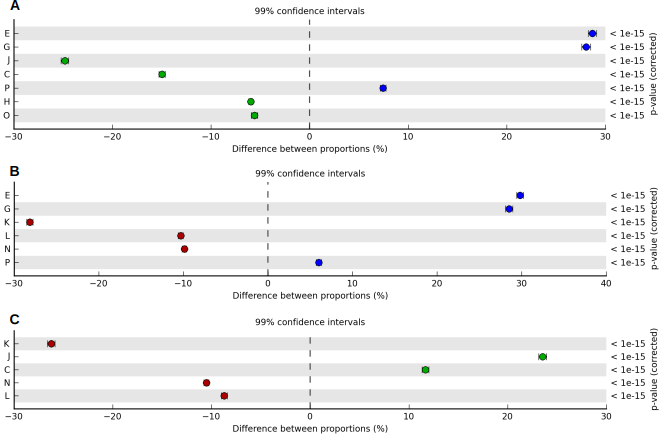
\includegraphics[width=\textwidth]{ace_figures/stamp.pdf}
\caption[Statistical analysis of Ace Lake metaproteome]{ Statistical analysis of normalised mass spectra from \ac{COG} annotated protein between each zone in Ace Lake. 
Proteins are shown grouped into \ac{COG} categories.
Only categories with corrected p-values $<$0.05 and effect size $>$5 are displayed.
(\textbf{A}) Mixolimnion compared to chemo/oxycline. 
(\textbf{B}) Mixolimnion compared to monimolimnion.
(\textbf{C}) Chemo/oxycline compared to monimolimnion. 
Blue, mixolimnion; green, interface; red, monimolimnion.
\ac{COG} category descriptions are: E, amino acid transport and metabolism; G, carbohydrate transport and metabolism; J, translation, ribosomal structure and biogenesis; C, energy production and conservation; P, inorganic ion transport and metabolism; H, co-enzyme transport and metabolism; O, post-translational modification, protein turnover and chaperones; K, transcription; L, replication, recombination and repair; N, cell motility.
}
\label{fig:stamp}

\end{figure}

This gave an indication of how functional processes were separated with depth.
Large numbers of functionally annotated proteins could also be clearly linked to taxonomic groups allowing their contribution to lake ecosystem function and their evolution within the Ace Lake community to be inferred.

\subsubsection{Mixolimnion}
The most abundant proteins in the mixolimnion were assigned to transport functions from COG categories (E) amino acid transport and metabolism, (G) carbohydrate transport and metabolism and (P) inorganic ion transport and metabolism \figref{fig:stamp}. 
Most of the protein identifications could be related to taxonomic groups as well as protein families.
The transporters were predominately \ac{ABC} type, with a high \ac{COG} representation of transporters for carbohydrates ($\sim$34\% of normalised spectra), amino acids ($\sim$32\%) and inorganic ions ($\sim$9\%) (\figreft{fig:stamp}, \tabreft{tab:ace_protids_5m}, \tabreft{tab:ace_protids_11.5m} ).
The prevalence of amino acid and simple sugar transporters and the low \ac{DOC} concentration in the Ace Lake mixolimnion \figref{fig:ace_diagram} is likely to reflect efficient utilisation of these substrates from the \ac{DOC} pool.
Thus, examination of the expressed transport proteins may better indicate substrate preferences and nutritional requirements than measurements of nutrient availability. 

All transporters in the metaproteome were of bacterial origin and conservative phylum level assignments of the normalised spectral abundance showed the majority to originate from \emph{Proteobacteria} (69\%), of which SAR11 comprised 46\% and \emph{Actinobacteria} 19\% (\tabreft{tab:ace_protids_5m}, \tabreft{tab:ace_protids_11.5m}). 
A high proportion of expressed genes with transport functions have also been reported for SAR11 from coastal \cite{Poretsky2010} and open ocean waters \cite{Sowell2009, Morris2010}. 
Oligotrophs, such as SAR11 not only posses a low-diversity of high-affinity transporters \cite{Lauro2009}, but regulate the relative abundance of transporters expressed in response to \ac{DOC} availability \cite{Poretsky2010}. 
The transporter expression profile of the Ace Lake SAR11 was very similar to that of the SAR11 in the Sargasso Sea \cite{Sowell2009}.
Two SAR11 transport proteins that were detected in Ace Lake (\tabreft{tab:ace_protids_5m}, \tabreft{tab:ace_protids_11.5m}) were not detected in the Sargasso Sea \cite{Sowell2009}: an ectoine/hydroxyectoine (167807477 and 167892279) and a zinc \ac{ABC} transporter (167933120). 
Ectoine is a compatible solute and presence of the ectoine transporter indicates it is more availible in Ace Lake than in the ocean, potentially in response to higher variability in salinity or low temperature.
The zinc \ac{ABC} transporter is likely to support zinc efflux in response to zinc concentrations which are $\sim$70-fold higher in the mixolimnion of Ace Lake compared to seawater \cite{Rankin1999}. 
Conversely, phosphate transporters were a major class detected from the Sargasso Sea \cite{Sowell2009} but were absent from the Ace Lake metaproteome consistent with lower phosphate levels in the Sargasso Sea ($<$5 nM) compared to Ace Lake (1--12 \textmu{}M). 
The differences in transporter expression between Ace Lake and oceanic SAR11 are likely to signify adaptive growth strategies that have evolved in the Ace Lake SAR11 community.

\emph{Actinobacteria} sequences were associated with a diverse phylogenetic cluster (Luna cluster) mainly represented by freshwater ultramicrobacteria \cite{Hahn2003}. 
Several Luna cluster isolates contain rhodopsin genes, termed actinorhodopsins \cite{Sharma2009} and similar gene sequences were present in the Ace Lake oxic zone data and found to be expressed (167820670 and 163154474; \tabreft{tab:ace_protids_5m}, \tabreft{tab:ace_protids_11.5m}).
This was the first report of expression of these actinorhodopsin sequences.
The abundance of \emph{Actinobacteria} transporters along with their small cell size and distribution in the water column indicates they occupies a similar ecological niche as SAR11.
SAR11 contains proteorhodopsin which is a related to actinorhodopsin \cite{Sharma2009}.
Although the physiological role of proteorhodopsin in SAR11 is yet to be fully elucidated \cite{Fuhrman2008}, this provides some indication actinorhodopsins in Antarctic Luna cluster \emph{Actinobacteria} have a related functional role.

\subsubsection{Chemo/oxycline}
Proteins from the chemo/oxycline were almost all of \ac{GSB} origin \tabref{tab:ace_protids_12.7m}. 
An in-depth metaproteogenomic analysis of the \ac{GSB} metabolism has been described \cite{Ng2010a, Ng2010b}.
Comparative analysis of proteins between the lake strata showed this depth was more similar to the monimolimnion that the mixolimnion \figref{fig:stamp}.
Compared with the mixolimnion, \ac{COG} categories (J) translation, ribosomal structure and biogenesis; (C) energy production and conservation; (H) co-enzyme transport and metabolism and (O) post-translational modification, protein turnover and chaperones were overrepresented, whereas in comparison with the monimolimnion, only categories J and C were significantly overrepresented.
This difference likely due to the presence of sedimenting \ac{GSB} cells in the monimolimnion.
Nonetheless, overrepresentation of J and C categories indicates it is the \ac{GSB} population at the chemo/oxycline that is the most metabolically active and productive in the whole lake community.
The overrepresentation of category C is similarly evident in the metagenomic comparison of functional genes whereas category J is not \cite{Lauro2011}.
This indicates differences in the regulation of energy metabolism compared to protein translation in \ac{GSB}.

Both metagenomic and microscopic analysis of the \ac{GSB} layer has indicated the population lacks viruses.
Mathematical modeling predicted that the absence of virus predation in the \ac{GSB} could be an adaptation to longer cycles of growth and inactivity in response to the polar light regime \cite{Lauro2011}. 
A mechanism for how virus resistance may be conferred in the population was suggested in the metaproteome.
Abundant \ac{CRISPR} associated \ac{CAS} proteins Cse2, Cse3 and Cse4 (165526330, 165526332 and 165526334, respectively) were detected in the 12.7 m metaproteome \tabref{tab:ace_protids_12.7m}. 
The \ac{CAS} gene locus (cas3, cse1, cse2, cse3, cse4, cas5, cas1b), to which the proteins map, shares its organisation with \ac{CAS} loci of sequenced \ac{GSB}, and groups with the \emph{E. coli} subtype/variant 2. 
The \ac{CRISPR}/\ac{CAS} system has been shown in other organisms to mediate virus resistance \cite{Karginov2010, Horvath2010} and is likely to have a similar function in the Ace Lake \ac{GSB}.


\subsubsection{Monimolimnion}
In parallel with taxonomic diversity increasing with depth, with the exception of the \ac{GSB} layer, the rate of metaproteomic identification of proteins decreased with depth \tabref{tab:protid_stats}.
This is to be expected as complete coverage of all genomic information from an environment is unlikely from all but the most simple of systems which means that as diversity increases there is a greater chance a protein will map to fragmentary or absent metagenomic data and fail to be identified.
Annotated proteins in the monimolimnion were overrepresented in \ac{COG} categories (K) transcription; (L) replication, recombination and repair and (N) motility \figref{fig:stamp}. 
Categories L and N were similarly overrepresented in the monimolimnion metagenomic samples \cite{Lauro2011} demonstrating the genomic expansion of these functions correlated with higher abundance of these proteins.
However, differential adundance was greatest in the category K proteins, which showed showed little difference in relative abundance in the metagenomes \cite{Lauro2011} suggesting transcription proteins in the monimolimnion were up-regulated \figref{fig:stamp}. 
The majority of the proteins that were detected in the monimolimnion (e.g. 67\% at 23 m) \tabref{tab:ace_protids_23m} were for hypothetical proteins that tended to lack orthologues in well-characterized organisms.
This demonstrates the extremely high level of functional novelty in the anaerobic zone of the lake.
These hypothetical proteins represent potential targets for protein expression studies to determine their biological function.


%--------------------------------------------------------------------------------------------
\section{Conclusions}
This study has developed modifications to existing epifluorescence microscopy and metaproteomic methodologies that were successfully applied to the analysis of Ace Lake.
These methods provide independent datasets that complemented metagenomic sequencing.
The epifluorescence microscopy methodology was able to determine the relative difference in cell and \acp{VLP} down the lake profile and may prove to be a viable alternative to Anodisc-based protocols.
Modifications in the bioinformatic analysis of mass spectral data afforded an increase in the number of protein identifications by using the matched metagenome data, identified proteins with shared peptides and enabled estimation of protein abundances by spectral counting.
Both these methodologies have lent crucial bits of data to the integrative understanding of the whole lake ecosystem.
These included validating differences in the microbial community with size and depth, supporting the absence of viruses in the \ac{GSB} layer, trophic status of the lack, describing the transport functions in the lake surface and a potential mechanism for virus resistance in the \ac{GSB}.


%--------------------------------------------------------------------------------------------
\section{Acknowledgements}
This work was supported by the Australian Research Council, the Australian Antarctic Division, the University of New South Wales and the \textsc{NSW} Government. 
The work contributed by members of the \ac{JCVI} was supported by funding from the Gordon and Betty Moore Foundation.
Mass spectrometry and analysis was conducted at the Bioanalytical Mass Spectrometry Facility at the Analytical Centre of \textsc{UNSW}.
